\documentclass[aspectratio=43, xcolor=table]{beamer}
\usepackage{../../preamble_math}
\usepackage{subcaption}

%%%%%% Logo definitions %%%%%%
\def\logoconference{tsfp.png/1.5cm/-0.3cm} % conference logo
% logo path / logo height / logo yshift
\def\institutionlogos{ICL_Logo_Blue_CMYK.pdf/0.4cm/0.3cm,boeing.pdf/0.85cm/0cm}
\def\separation{0.7cm}
%%%%%%%%%%%%%%%%%%%%%%%%%%%%%%

%%%%%% Custom colors %%%%%%
\definecolor{customcolor}{RGB}{3, 75, 152}
%%%%%%%%%%%%%%%%%%%%%%%%%%%

%%%%%% Load custom styling %%%%%%
\usepackage{../../myImperialBeamerTemplate}
%%%%%%%%%%%%%%%%%%%%%%%%%%%%%%

%%%%%%% Metadata %%%%%%%
\title{Effects of Mach number and 3D instabilities on boundary-layer transition over gaps}
\author{Víctor Ballester Ribo, Jeffrey Crouch, Yongyun Hwang, Spencer Sherwin}
\author{
	\texorpdfstring{\underline{Víctor Ballester Ribó}$^1$, Jeffrey Crouch$^2$, \\
	Yongyun Hwang$^1$, Spencer Sherwin$^1$}{}
}
\institute{
  $^1$Department of Aeronautics, Imperial College London, UK \\
  $^2$The Boeing Company, USA
}
\date{29 July 2026}
%%%%%%%%%%%%%%%%%%%%%%%%%%


\begin{document}

\begin{frame}\titlepage\end{frame}

\begin{frame}{Motivation}
	\begin{figure}
		\centering
		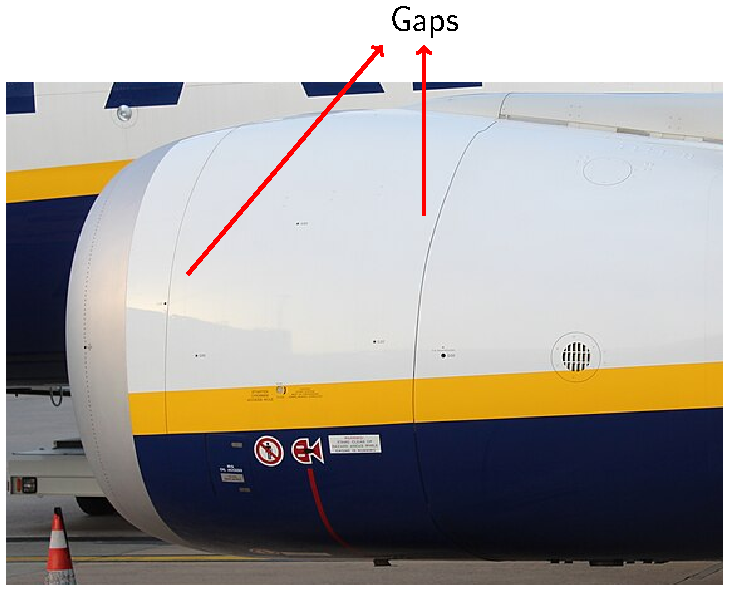
\includegraphics[width=0.8\linewidth]{Images/nacelle.pdf}
		\caption{Engine nacelle of a Boeing 737}
	\end{figure}
\end{frame}
\begin{frame}
	\frametitle{First questions}
	\begin{itemize}
		\item Small disturbances in the boundary layer initially grow as $\propto \exp{n(x)}$.
		\item We aim to understand how much a gap of width $w$ and depth $d$ can overamplify these disturbances.
		\item For each gap of width $w$ and depth $d$, we define $$\Delta n_{\text{gap}} := n_\text{gap} - n_\text{flat}$$
	\end{itemize}
\end{frame}
\begin{frame}
	\frametitle{Experimental observations}
	\begin{columns}[T] % [T] ensures correct vertical alignment
		\begin{column}{0.49\linewidth} % left column
			\begin{figure}
				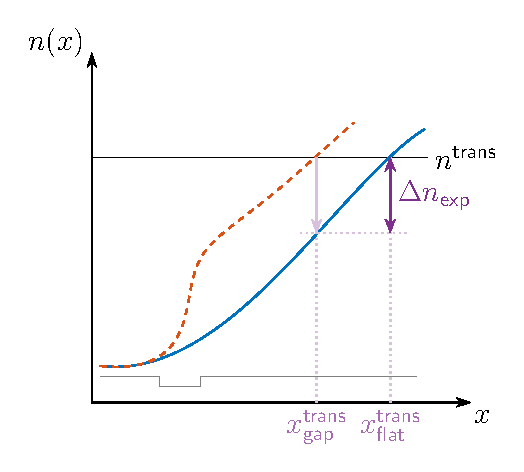
\includegraphics[width=\textwidth]{Images/amplificationQualititiveNfactorOnlyExp.pdf}
			\end{figure}
		\end{column}
		\begin{column}{0.49\linewidth} % left column
			\begin{figure}[ht]
				\centering
				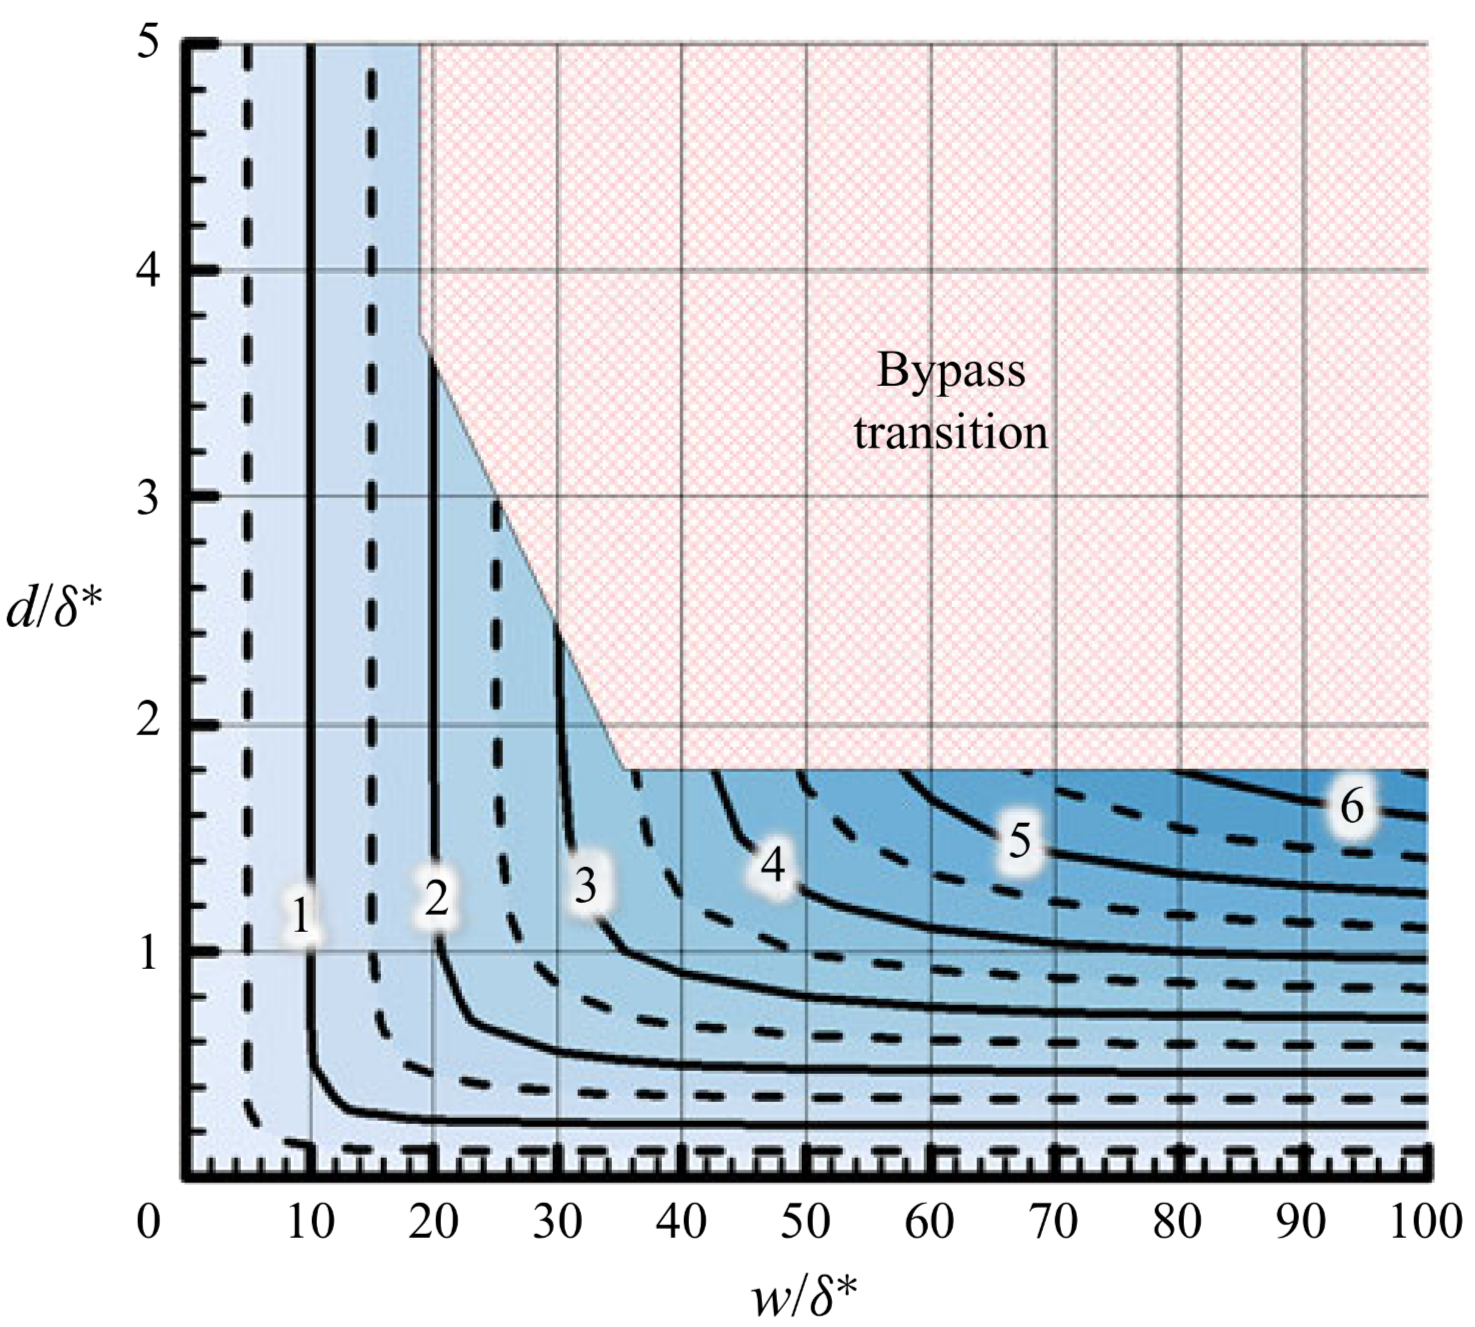
\includegraphics[width=\textwidth]{Images/deltaNfactorsJeff.png}
				\caption{$\Delta n_{\text{gap}}$ contours in the $w$-$d$ parameter space, from experiments by Crouch et al. (2022)${}^\dag$.}
			\end{figure}
		\end{column}
	\end{columns}
	{\fontsize{6}{8}\selectfont
	\textit{${}^\dag$Crouch JD, Kosorygin VS, Sutanto MI, Miller GD. Characterizing surface-gap effects on boundary-layer transition dominated by Tollmien–Schlichting instability. Flow. 2022;2:E8.}}
\end{frame}
\begin{frame}{Numerical setup}

	\begin{figure}[ht]
		\centering
		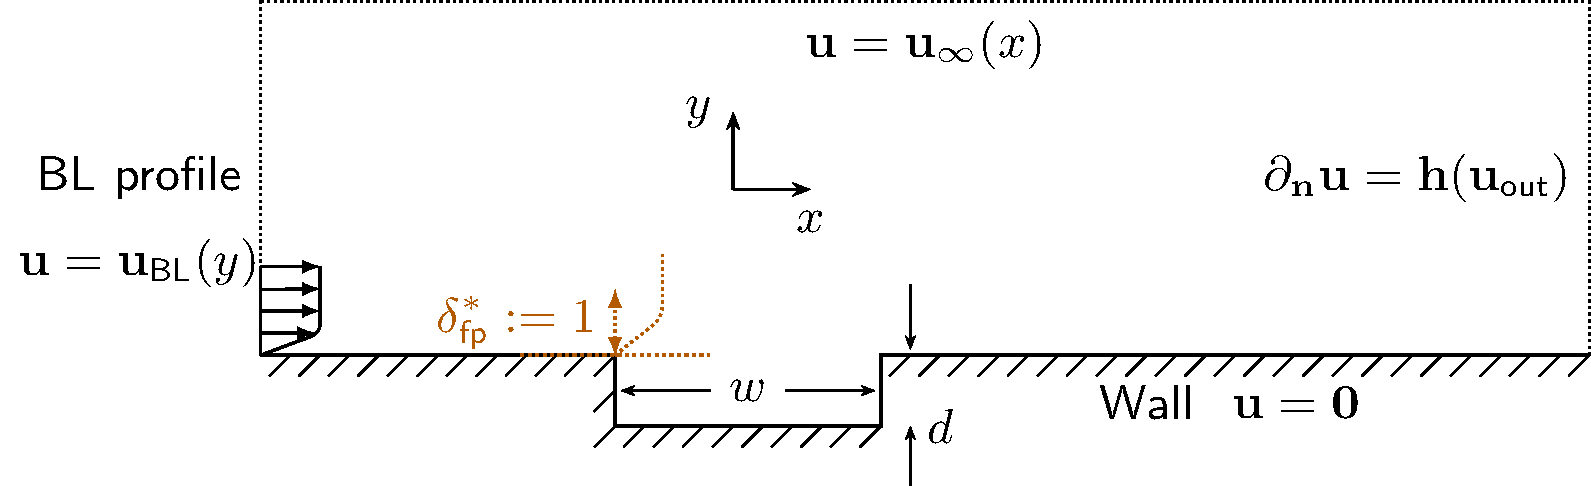
\includegraphics[width=\textwidth]{Images/domainBaseflowExtended.pdf}
		\caption{Domain setup for the steady-state finder }
	\end{figure}
	\textbf{Aims:}
	\begin{itemize}
		\item Study the stability of the system as a function of the depth $d$ and width $w$ of the gap. Reynolds number is fixed to
		      $$\Rey= \frac{u_\infty \delta^*_\text{fp}}{\nu} = 1000.$$
		\item Understand the influence of the Mach number.
		\item To what extend are 3D effects important?
	\end{itemize}

\end{frame}
\begin{frame}{2d incompressible limit set classification}
	\begin{figure}
		\centering
		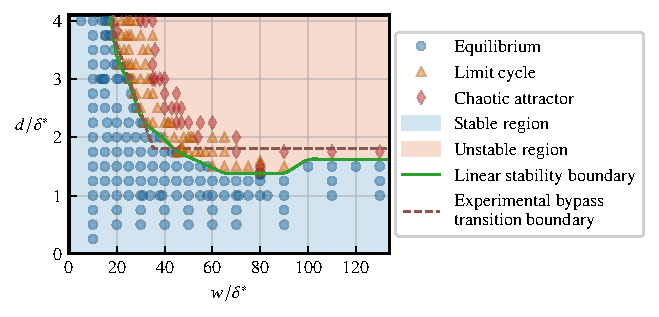
\includegraphics{Images/inc2dStabilityCurveRe1000.pdf}
		\caption{Limit set classification over the parameter space $10 \leq w/\delta^*\leq 130$ and $0.25 \leq d/\delta^*\leq 4$.}
	\end{figure}
\end{frame}
\begin{frame}
	\frametitle{Stability setup to excite the boundary layer}
	\begin{columns}[T] % [T] ensures correct vertical alignment
		\begin{column}{0.4\linewidth} % left column
			\begin{itemize}
				\item We linearize the flow around a steady base flow.
				\item We add a stochastic forcing term in the upstream part of the boundary layer as a form of white Gaussian noise.
			\end{itemize}
		\end{column}
		\begin{column}{0.59\linewidth} % left column
			\begin{figure}[ht]
				\centering
				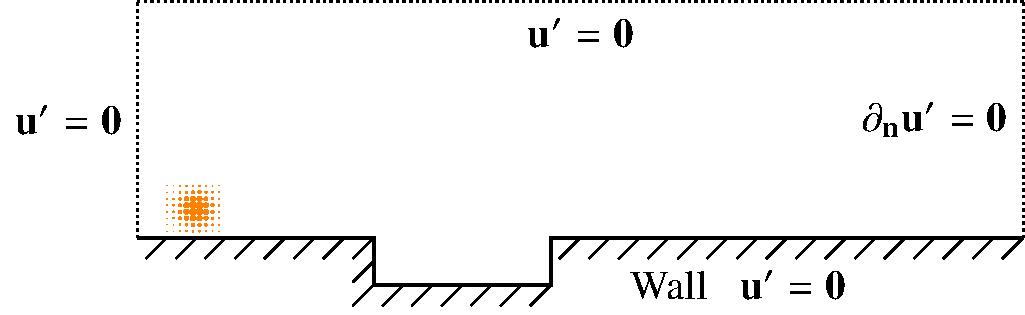
\includegraphics[width=\linewidth]{Images/domainPert.pdf}
			\end{figure}
			\vspace{-0.75cm}
			\begin{figure}[ht]
				\centering
				\includegraphics[width=\linewidth]{Images/amplificationQualititiveNfactor.pdf}
				% \includegraphics[width=\linewidth]{../../Images/amplificationQualititiveNfactor.pdf}
			\end{figure}
		\end{column}

	\end{columns}
\end{frame}
\begin{frame}
	\frametitle{$n$-factor curves}
	\begin{columns}[T] % [T] ensures correct vertical alignment
		\begin{column}{0.48\linewidth} % left column
			\textbf{Evolution of $n$ for disturbances growing as $\propto \exp{n(x)}$}
			\begin{figure}[ht]
				\centering
				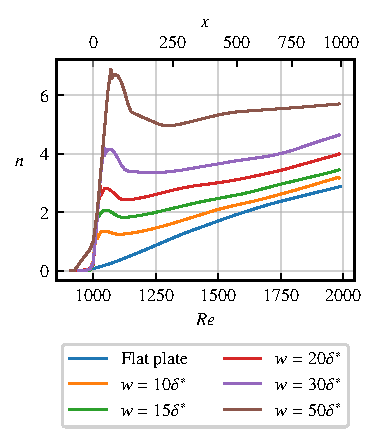
\includegraphics[width=\linewidth]{Images/nfactorCurvesd1.5.pdf}
			\end{figure}
		\end{column}
		\begin{column}{0.48\linewidth} % left column
			\textbf{Spatial stability curves for the parallel flow assumption}
			\begin{figure}[ht]
				\centering
				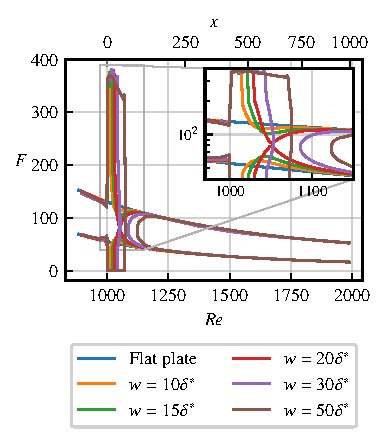
\includegraphics[width=\linewidth]{Images/neutrald1.5.pdf}
			\end{figure}
		\end{column}
	\end{columns}
\end{frame}

\begin{frame}{Numerical predictions of $\Delta n$}
	\begin{figure}
		\centering
		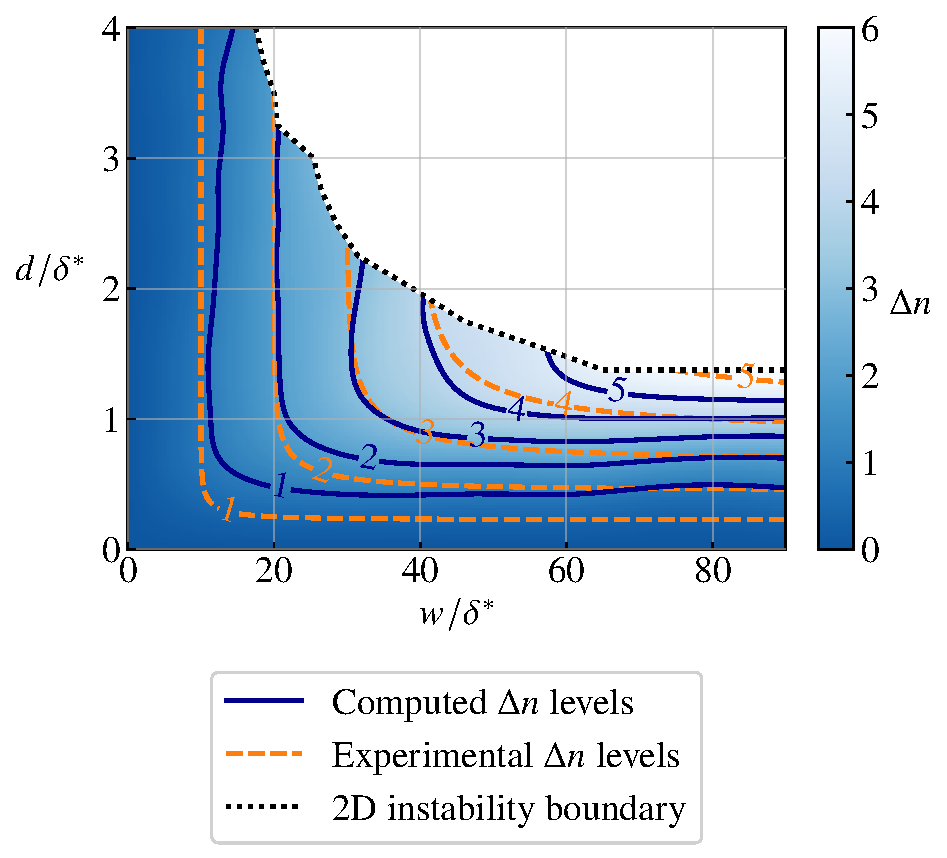
\includegraphics[width=0.7\textwidth]{Images/DeltaNcountour.pdf}
		\caption{Contours of $\Delta n$ in the $w$-$d$ parameter space.}
	\end{figure}
\end{frame}
\begin{frame}{3d effects}
	\begin{columns}[T] % [T] ensures correct vertical alignment
		\begin{column}{0.39\linewidth} % left column
			\begin{itemize}
				\item We perform single mode stability analysis to find the largest growth rate of 3D modes as a function of the spanwise wavenumber $\beta$.
			\end{itemize}
		\end{column}
		\begin{column}{0.7\linewidth} % left column
			\begin{figure}
				\centering
				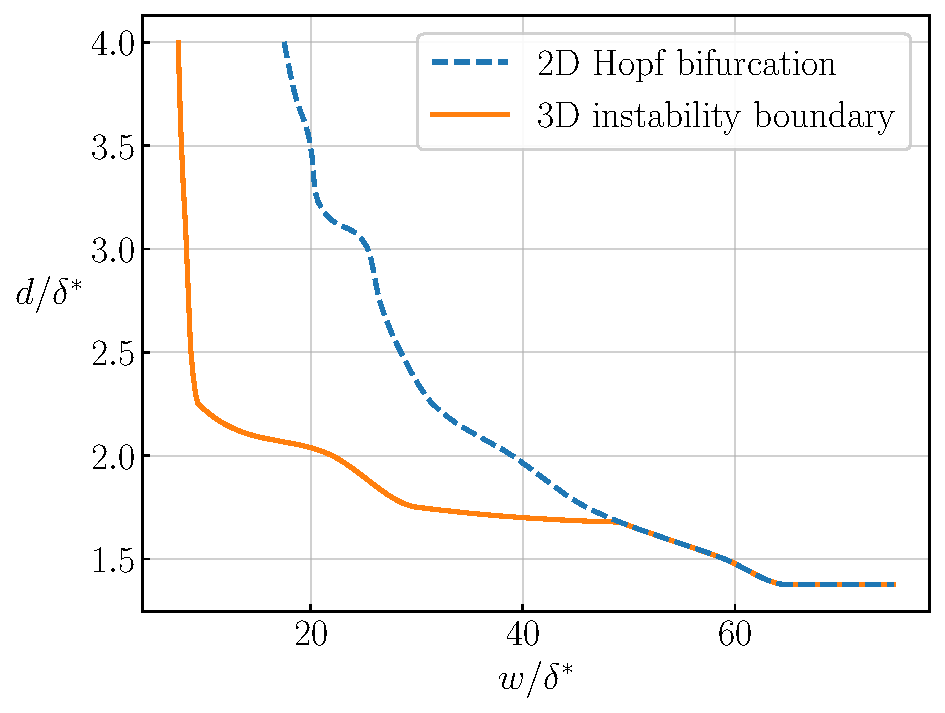
\includegraphics[width=\textwidth]{Images/3d2dbifurcations.pdf}
				\caption{Bifurcation boundaries for the 2D and 3D instabilities.}
			\end{figure}
		\end{column}
	\end{columns}
\end{frame}
\begin{frame}{3d non-linear results}
	\begin{columns}[T] % [T] ensures correct vertical alignment
		\begin{column}{0.45\linewidth} % left column
			\vspace{-0.5cm}
			\begin{figure}
				\centering
				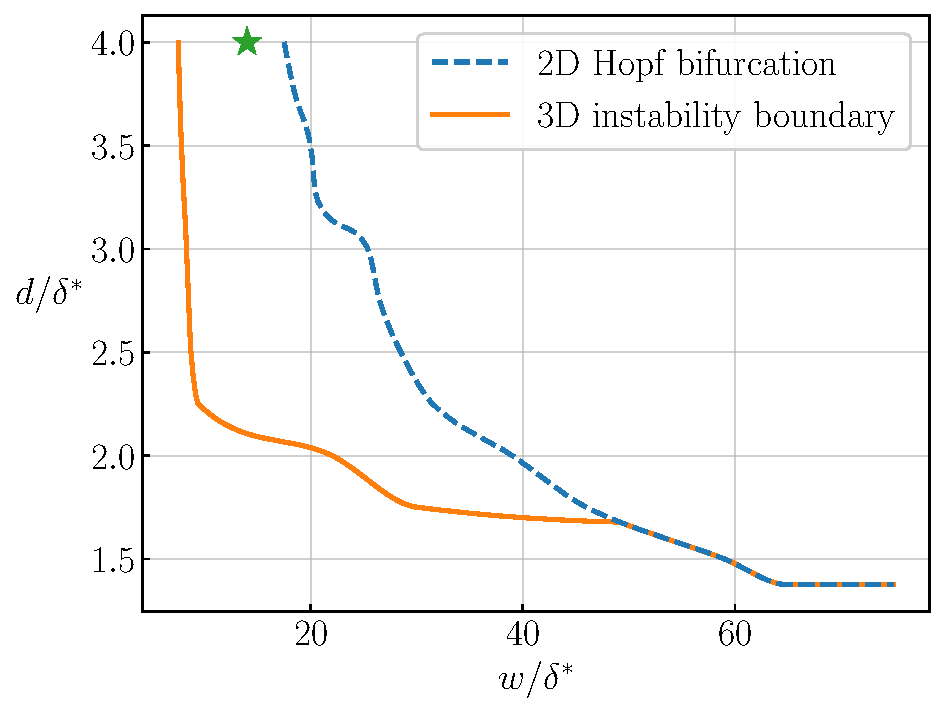
\includegraphics[width=1\textwidth]{Images/3d2dbifurcations_middleStar.pdf}
			\end{figure}
		\end{column}
		\begin{column}{0.55\linewidth} % left column
			{
				\begin{itemize}
					\item Long streaky structures appear in the downstream part of the gap
					\item Chaotic behaviour is observed in the gap, but insufficient to destabilise the system.
				\end{itemize}
			}
		\end{column}
	\end{columns}
	\begin{figure}[ht]
		\vspace{-2cm}
		{
		\hspace*{3cm}
		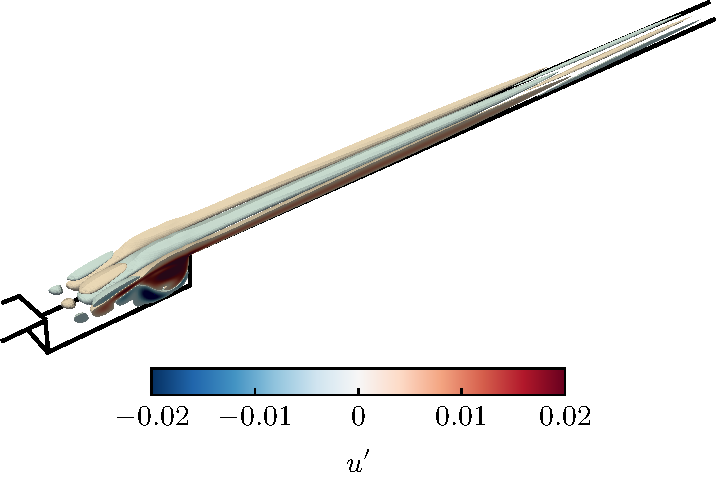
\includegraphics[width=0.7\linewidth]{Images/3dmode.pdf}
		\vspace{-0.3cm}
	\caption{Most unstable mode for the 3D instability.}}
	\end{figure}
\end{frame}
\begin{frame}{3d transition}
	\begin{columns}[T] % [T] ensures correct vertical alignment
		\begin{column}{0.4\linewidth} % left column
			\vspace{-0.5cm}
			\begin{figure}
				\centering
				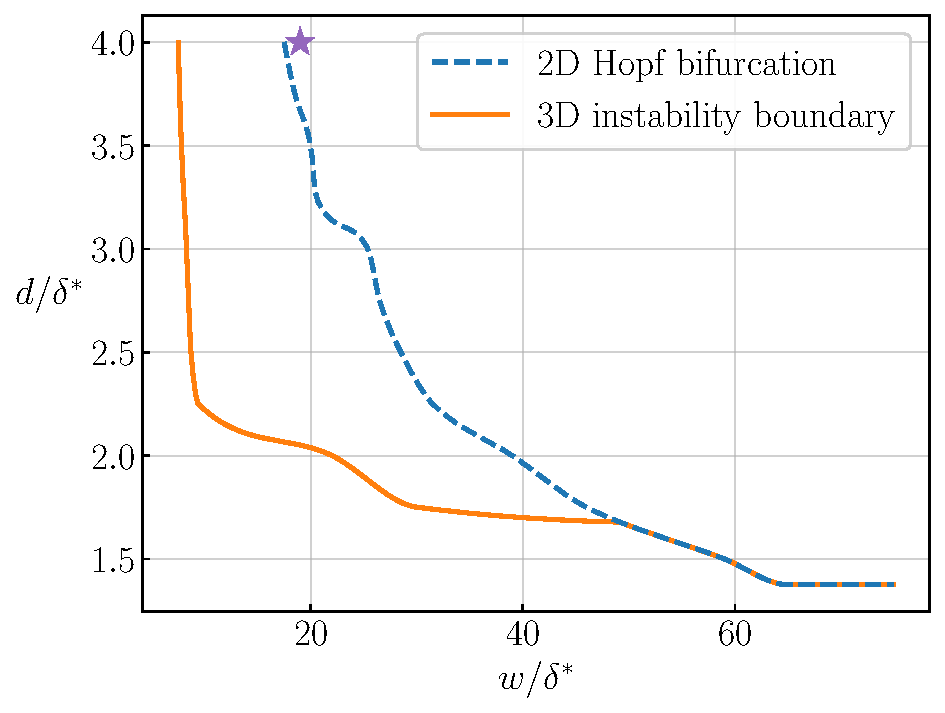
\includegraphics[width=1.1\textwidth]{Images/3d2dbifurcations_rightStar.pdf}
			\end{figure}
			\begin{figure}
				\makebox[\linewidth][l]{%
					\hspace{0.3cm}
					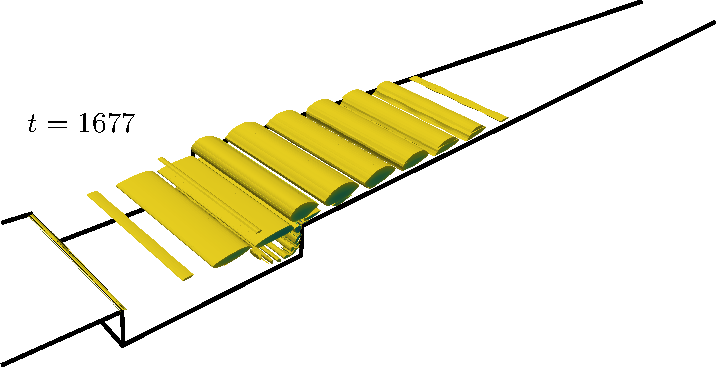
\includegraphics[width=1.185\linewidth]
					{Images/d4w19_3d_L2crit_10.pdf}
				}
			\end{figure}
		\end{column}
		\begin{column}{0.79\linewidth} % left column
			\vspace{-1cm}
			\begin{figure}[ht]
				\centering
				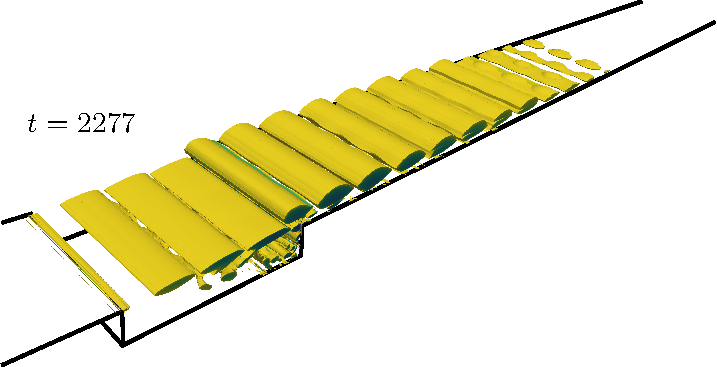
\includegraphics[width=0.6\linewidth]{Images/d4w19_3d_L2crit_12.pdf}
			\end{figure}
			\vspace{-2cm}
			\begin{figure}[ht]
				\centering
				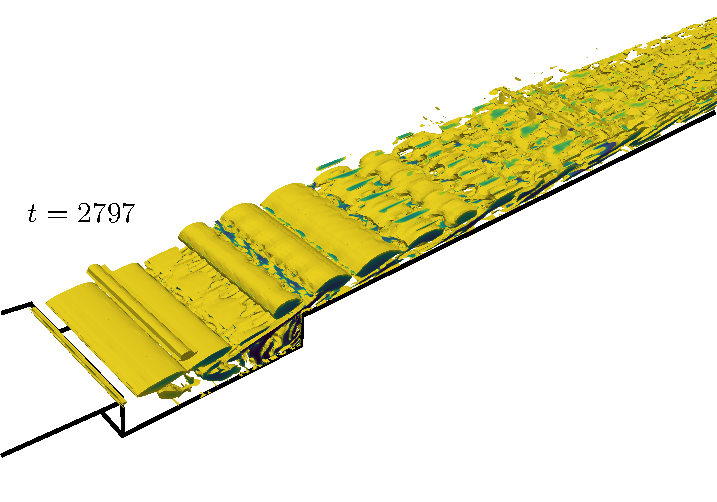
\includegraphics[width=0.6\linewidth]{Images/d4w19_3d_L2crit_14_big.pdf}
			\end{figure}
			\vspace{-2.5cm}
			\begin{figure}[ht]
				\centering
				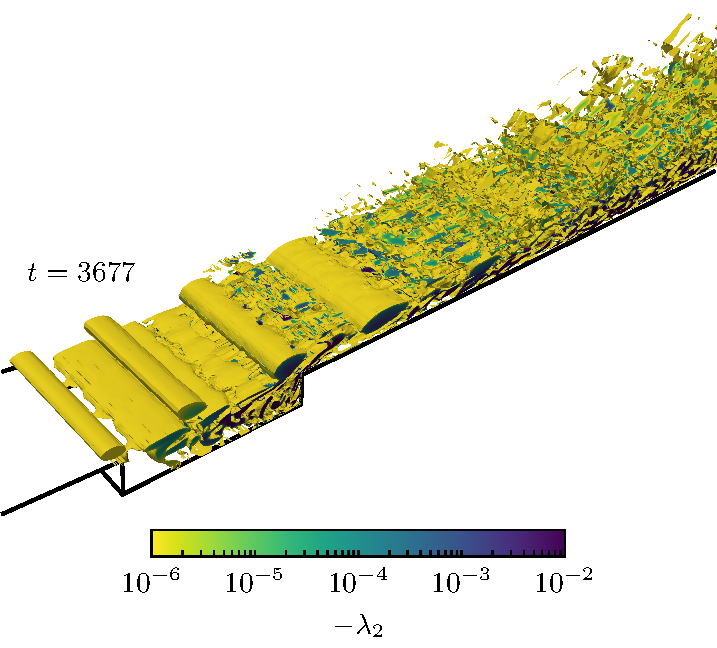
\includegraphics[width=0.6\linewidth]{Images/d4w19_3d_L2crit_17_big.pdf}
			\end{figure}
		\end{column}
	\end{columns}
\end{frame}
\begin{frame}{Mach number effects}

	\begin{figure}[ht]
		\centering
		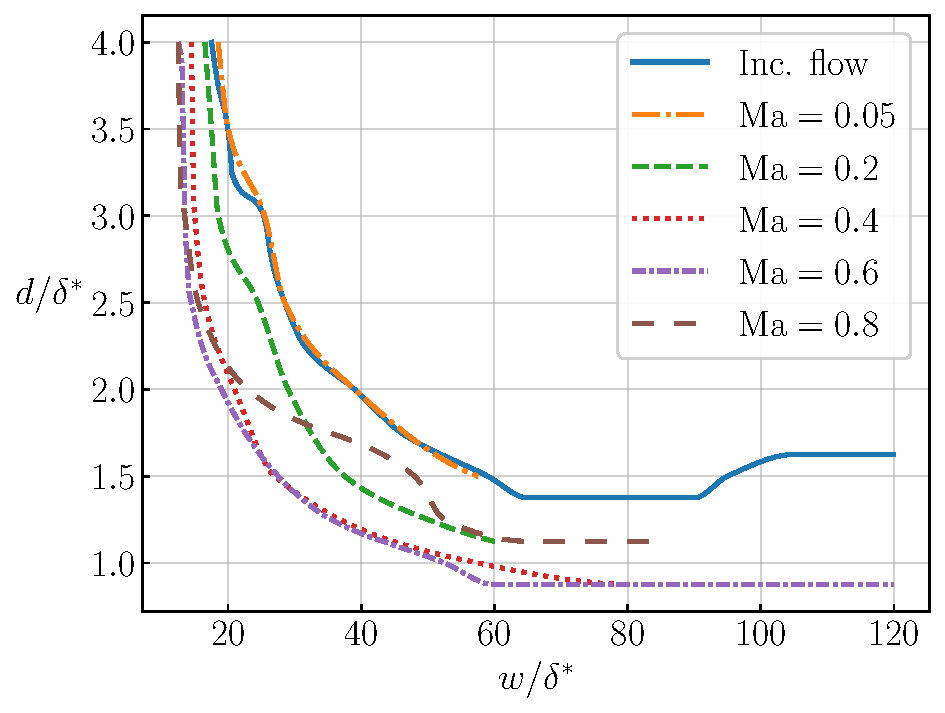
\includegraphics[width=0.7\textwidth]{Images/Mabifurcations.pdf}
		\caption{Hopf bifurcation boundaries for different Mach numbers.}
	\end{figure}

\end{frame}
\begin{frame}
	\frametitle{Conclusions}
	\begin{itemize}
		\item Very good agreement between the numerical predictions (2d inc.) and the experimental (3d low Mach wind tunnel) results.
		\item The 3D instability doesn't seem to be strong enough to destabilise the downstream boundary layer. Only after the 2D instability sets in, the transition location advances till the downstream edge of the gap.
		\item For deep gaps, Mach number has a destabilising effect, while for shallow gaps, higher Mach numbers lead to later transition.
	\end{itemize}
\end{frame}
\end{document}
